\documentclass[10pt]{beamer}

\usetheme[
%%% options passed to the outer theme
%    hidetitle,           % hide the (short) title in the sidebar
%    hideauthor,          % hide the (short) author in the sidebar
%    hideinstitute,       % hide the (short) institute in the bottom of the sidebar
%    shownavsym,          % show the navigation symbols
%    width=2cm,           % width of the sidebar (default is 2 cm)
%    hideothersubsections,% hide all subsections but the subsections in the current section
%    hideallsubsections,  % hide all subsections
    left               % right of left position of sidebar (default is right)
%%% options passed to the color theme
%    lightheaderbg,       % use a light header background
  ]{AAUsidebar}

% If you want to change the colors of the various elements in the theme, edit and uncomment the following lines
% Change the bar and sidebar colors:
%\setbeamercolor{AAUsidebar}{fg=red!20,bg=red}
%\setbeamercolor{sidebar}{bg=red!20}
% Change the color of the structural elements:
%\setbeamercolor{structure}{fg=red}
% Change the frame title text color:
%\setbeamercolor{frametitle}{fg=blue}
% Change the normal text color background:
%\setbeamercolor{normal text}{bg=gray!10}
% ... and you can of course change a lot more - see the beamer user manual.


\usepackage[utf8]{inputenc}
\usepackage{comment}
\usepackage{lmodern}
\usepackage{ucs}
\usepackage{t1enc}
\usepackage[english]{babel}
%\usepackage[T1]{fontenc}
% Or whatever. Note that the encoding and the font should match. If T1
% does not look nice, try deleting the line with the fontenc.
\usepackage{helvet}

\usepackage{subcaption}
\captionsetup{compatibility=false}

% colored hyperlinks
\newcommand{\chref}[2]{%
  \href{#1}{{\usebeamercolor[bg]{AAUsidebar}#2}}%
}


\date{}


	\title{PsyLog: Søvn og Aktivitetsmoduler for Personer med Affektive Lidelser}
	\author[sw808f15]{
			Lasse Vang Gravesen \\
			Søren Skibsted Als\\
			Lars Andersen \\
			Mathias Winde Pedersen
}
	
% - Give the names in the same order as they appear in the paper.
% - Use the \inst{?} command only if the authors have different
%   affiliation. See the beamer manual for an example




% specify a logo on the titlepage (you can specify additional logos an include them in 
% institute command below
\pgfdeclareimage[height=1.5cm]{titlepagelogo}{AAUgraphics/aau_logo_new} % placed on the title page
%\pgfdeclareimage[height=1.5cm]{titlepagelogo2}{graphics/aau_logo_new} % placed on the title page
\titlegraphic{% is placed on the bottom of the title page
  \pgfuseimage{titlepagelogo}
%  \hspace{1cm}\pgfuseimage{titlepagelogo2}
}

\graphicspath{ {Media/} }
\newcommand{\btVFill}{\vskip0pt plus 1filll}

\begin{document}
% the titlepage
{\aauwavesbg%
\begin{frame}[plain,noframenumbering] % the plain option removes the sidebar and header from the title page
  \titlepage
\end{frame}}
		

% includes her
\section{Introduktion}
\begin{frame}
\frametitle{PsyLog platformen}
	\begin{itemize}
	\item Modulær platform til indsamling og analyse af data
	\item Gør det nemt at udvikle moduler som tilbyder ny funktionalitet
	\item Fokus på mentalt helbred
	\item Præsentation i dag vil omhandle udvikling af moduler dertil
	\end{itemize}
\end{frame}

\section{Mentalt helbred}
\begin{frame}
\frametitle{Indikatorer på mentalt helbred}
	\begin{itemize}
	\item Ændring i søvnvaner og aktivitetsniveau
	\item Fokus på søvn, da søvn er noget af det mest centrale ifølge flere personer
	\item Hvad er søvn? % Søvn er en tilstand af hvile. Dette er karakteriseret af fuldt eller delvis tab af bevidsthed, så der er en nedsættelse af kropslig bevægelse og respons til stimulus. Formålet med søvn er blandt andet at få kroppens kræfter genoprettet.
	\item Søvn kan svinge i begge retninger: For lidt eller for meget
	\item God indikator for unipolar eller bipolar depression
	\end{itemize}
\end{frame}

\section{Soevn}
\begin{frame}
\frametitle{Krav til søvnestimering}
	\begin{itemize}
	\item Undgå brugerintervention
	\item Brug i eget hjem
	\item Være præcis
	\end{itemize}
\end{frame}

\section{Forarbejde til søvnestimering}
\begin{frame}
\frametitle{Metoder}
	\begin{itemize}
	\item Kan vi benytte eksisterende metoder?
	\item Hvilke metoder er der?
	{\begin{itemize}
		\item Polysomnografi
		\item Toss'N'Turn
		\item Best Effort Sleep
		 \end{itemize}}
	\end{itemize}
\end{frame}

\begin{frame}
\frametitle{Polysomnografi}
\begin{figure}
	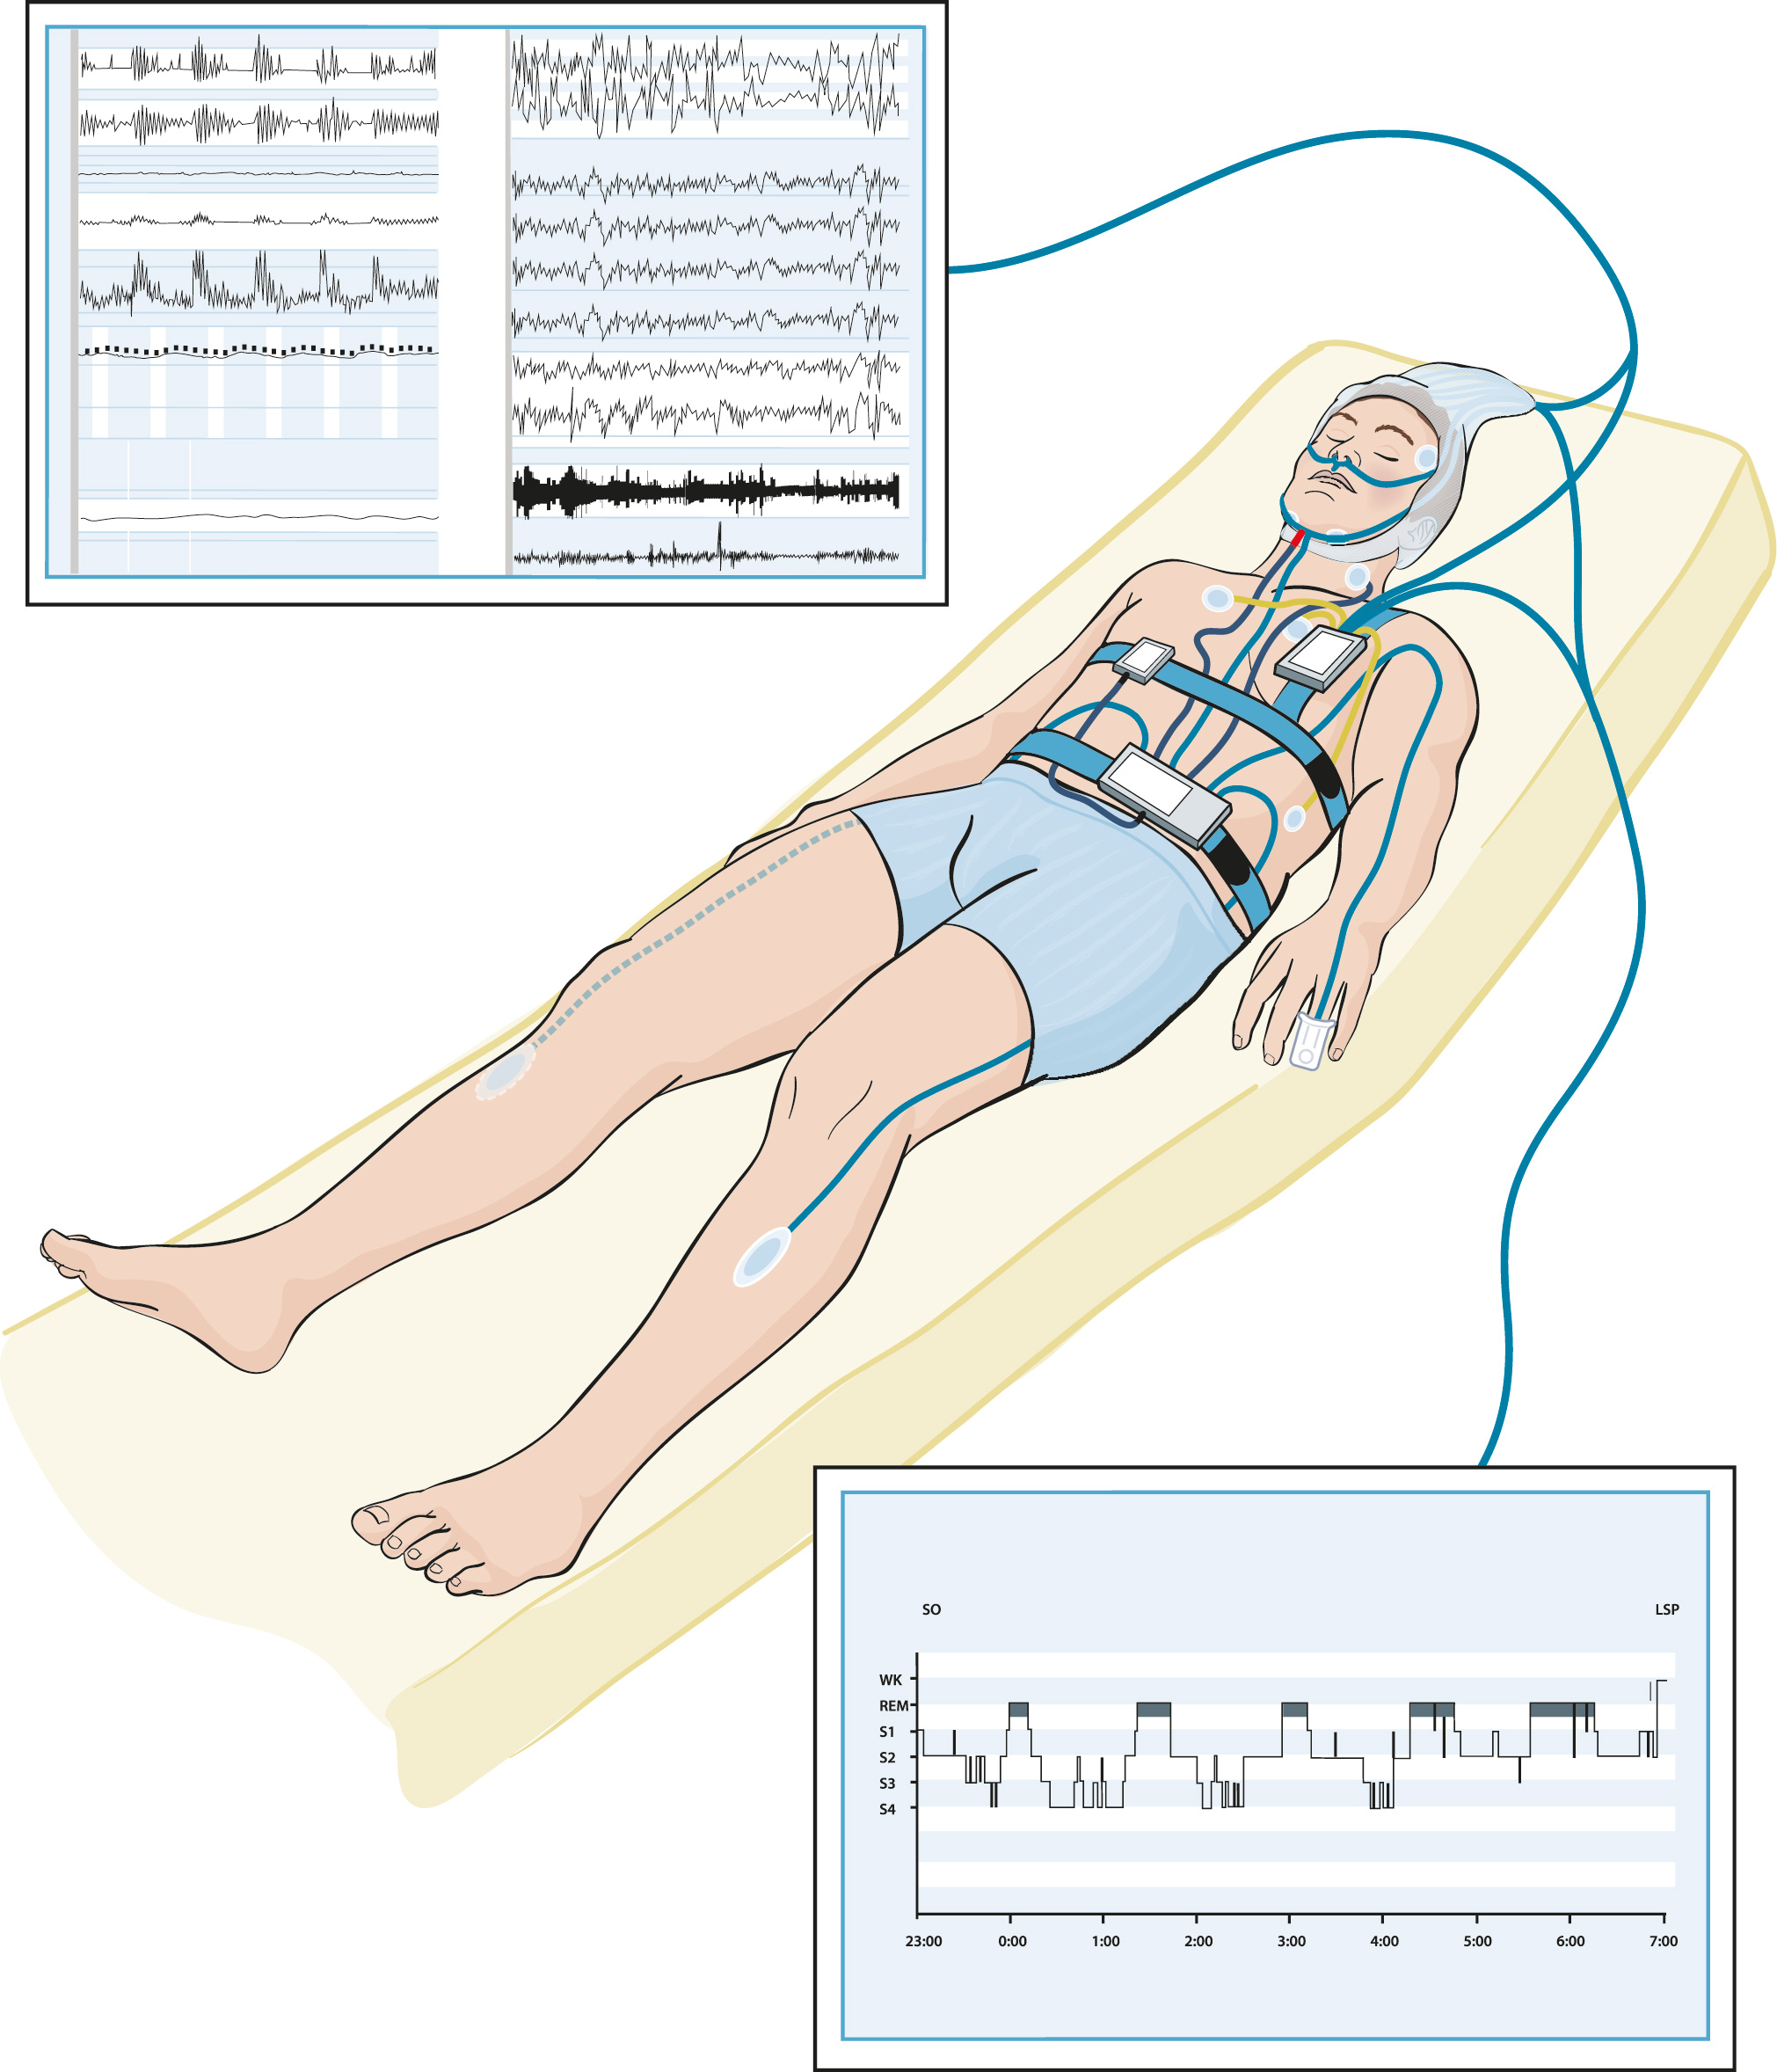
\includegraphics[scale=0.05]{polysomnografi}
\end{figure}

\begin{itemize}
	\item State of the art
	\item Kræver ekspert viden og specialudstyr og kan ikke bruges af en patient i eget hjem
\end{itemize}
\end{frame}

\begin{frame}
\frametitle{Toss'N'Turn}
\begin{itemize}
	\item 92\% nøjagtig søvnlængdeestimering
	\item Læringsperiode
\end{itemize}
\end{frame}

\begin{frame}
	\frametitle{Best Effort Sleep}
	\begin{itemize}
		\item 92\% nøjagtig søvnlængdeestimering
	\end{itemize}
\end{frame}

% Nu vil als så forsætte
\section{Overvejelser}

\begin{frame}
	\centering
	Overvejelser
\end{frame}

\begin{frame}
\frametitle{Snorken}
	\begin{quote}
	Snorken er en åndedrætsforstyrrelse, hvor drøbelen eller den bløde gane sættes i vibrationer af en blokering i luftvejene.
	Snorken er en særdeles udbredt søvnforstyrrelse.
	\end{quote}	

	\begin{itemize}
		\item Kan være stærkt signal på søvn
		\item Også tegn på dårlig søvn
		\item Hvordan ved man hvem der snorker?
	\end{itemize}
	\centering
	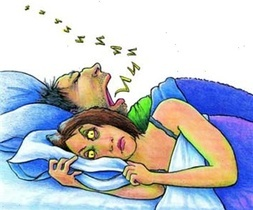
\includegraphics[scale=0.4]{snorken}
\end{frame}

\section{Proof of concept}

\begin{frame}
\frametitle{Proof of concept}
Vi betragter stilstandsperioder som indikator på søvn.

\begin{figure}
	\begin{minipage}{\linewidth}
		\begin{subfigure}{0.5\linewidth}
			\centering
			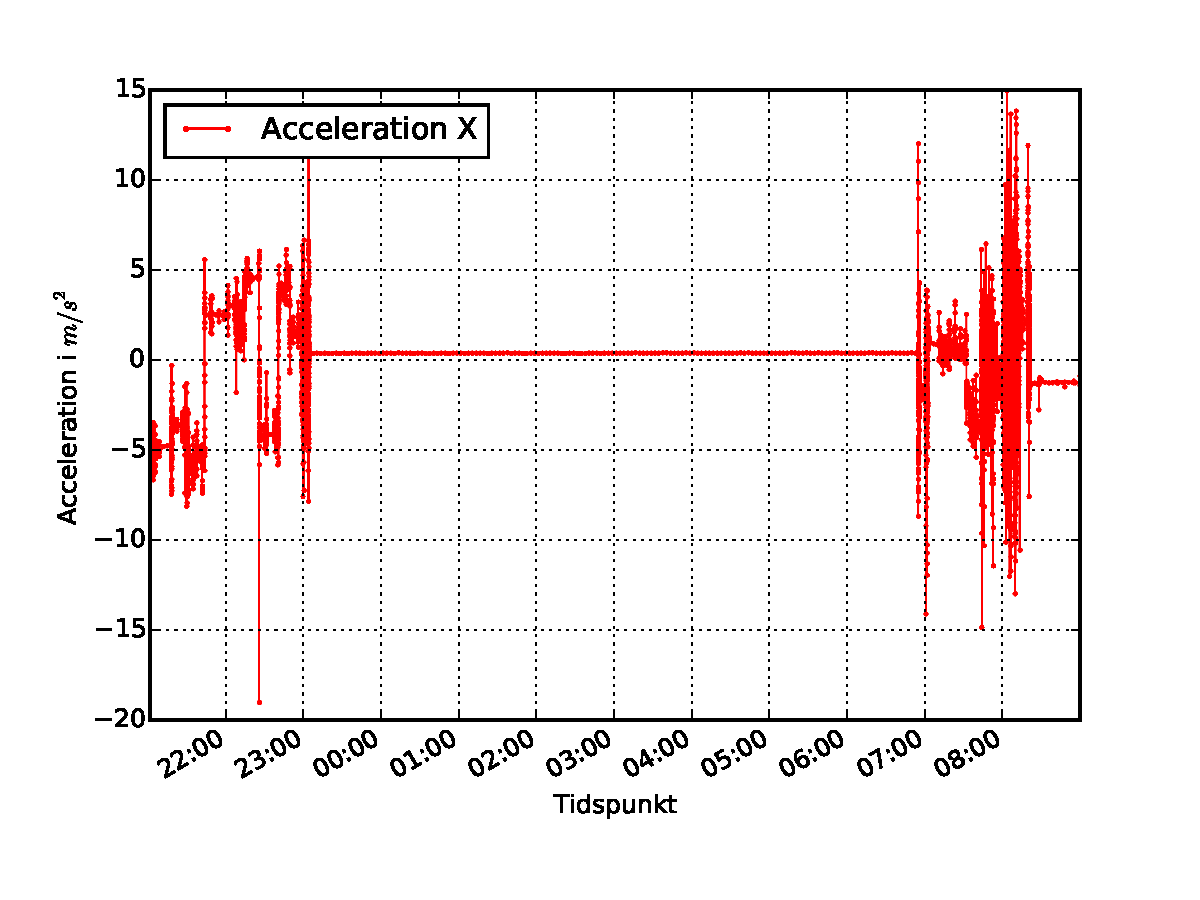
\includegraphics[scale=0.27, trim = 1cm 1cm 1cm 1cm, clip]{../Report/grafik/kombi_figur/acceleration-plot}
			\caption{Rå accelerations-data.}\label{fig:rawaccplot}
		\end{subfigure}
		\begin{subfigure}{0.5\linewidth}
			\centering
			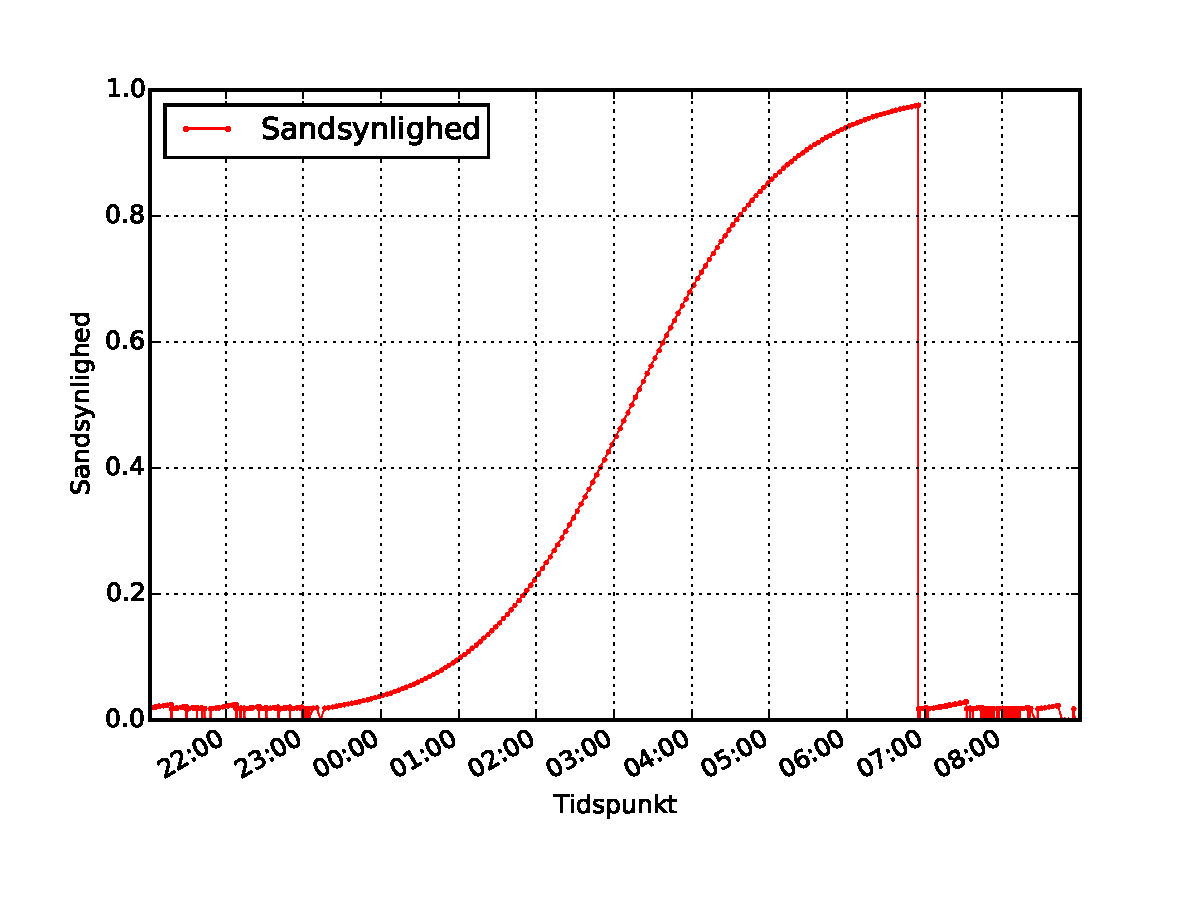
\includegraphics[scale=0.27, trim = 1cm 1cm 1cm 1cm, clip]{../Report/grafik/kombi_figur/acceleration-sleep-estimate-plot}
			\caption{Accelerations-søvnestimering.}\label{fig:sleepcalcaccplot}
		\end{subfigure}
	\end{minipage}\\[1ex]%
\end{figure}
\end{frame}

\begin{frame}
\frametitle{Proof of concept}
Vi betragter stilstandsperioder som indikator på søvn.

\begin{figure}
	\begin{minipage}{\linewidth}
		\begin{subfigure}{0.5\linewidth}
			\centering
			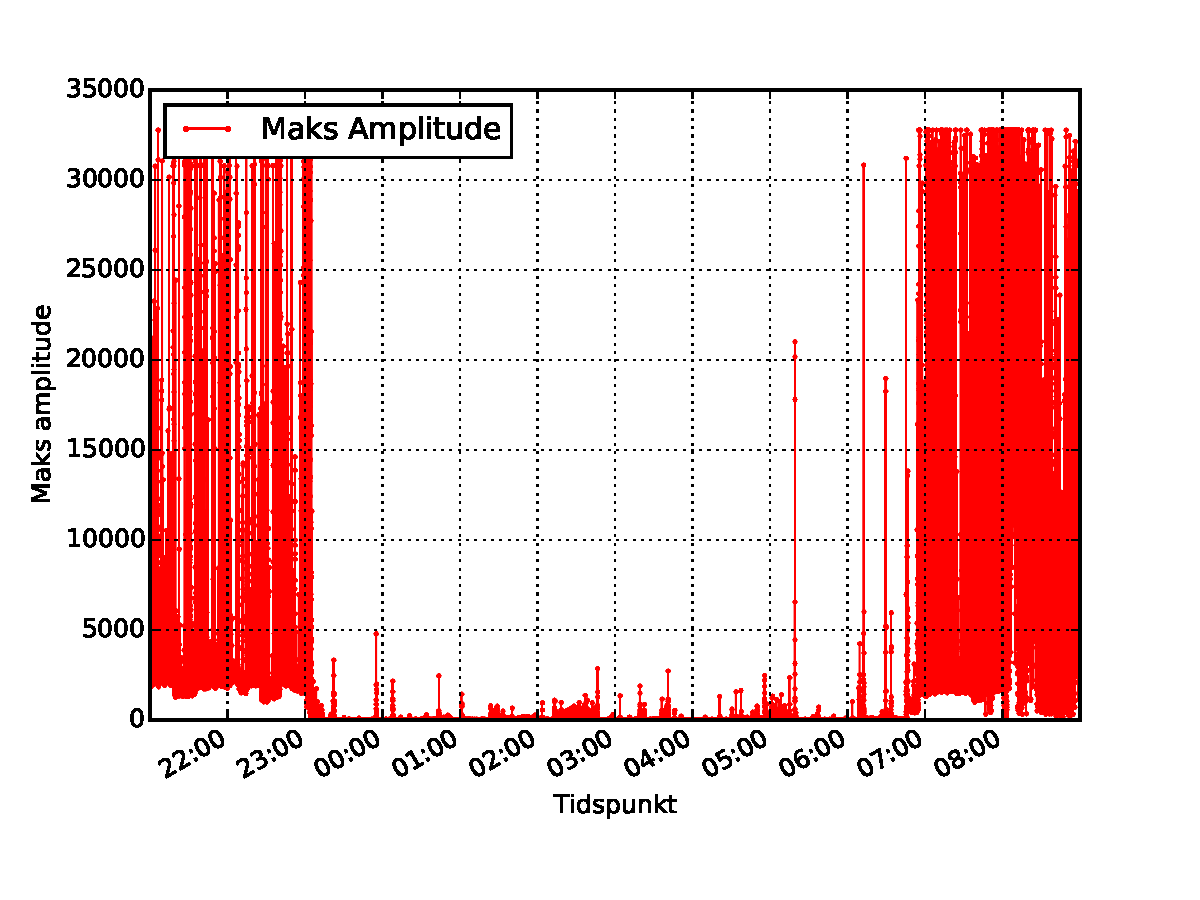
\includegraphics[scale=0.27, trim = 1cm 1cm 1cm 1cm, clip]{../Report/grafik/kombi_figur/amplitude-plot}
			\caption{Rå amplitude-data.}
		\end{subfigure}
		\begin{subfigure}{0.5\linewidth}
			\centering
			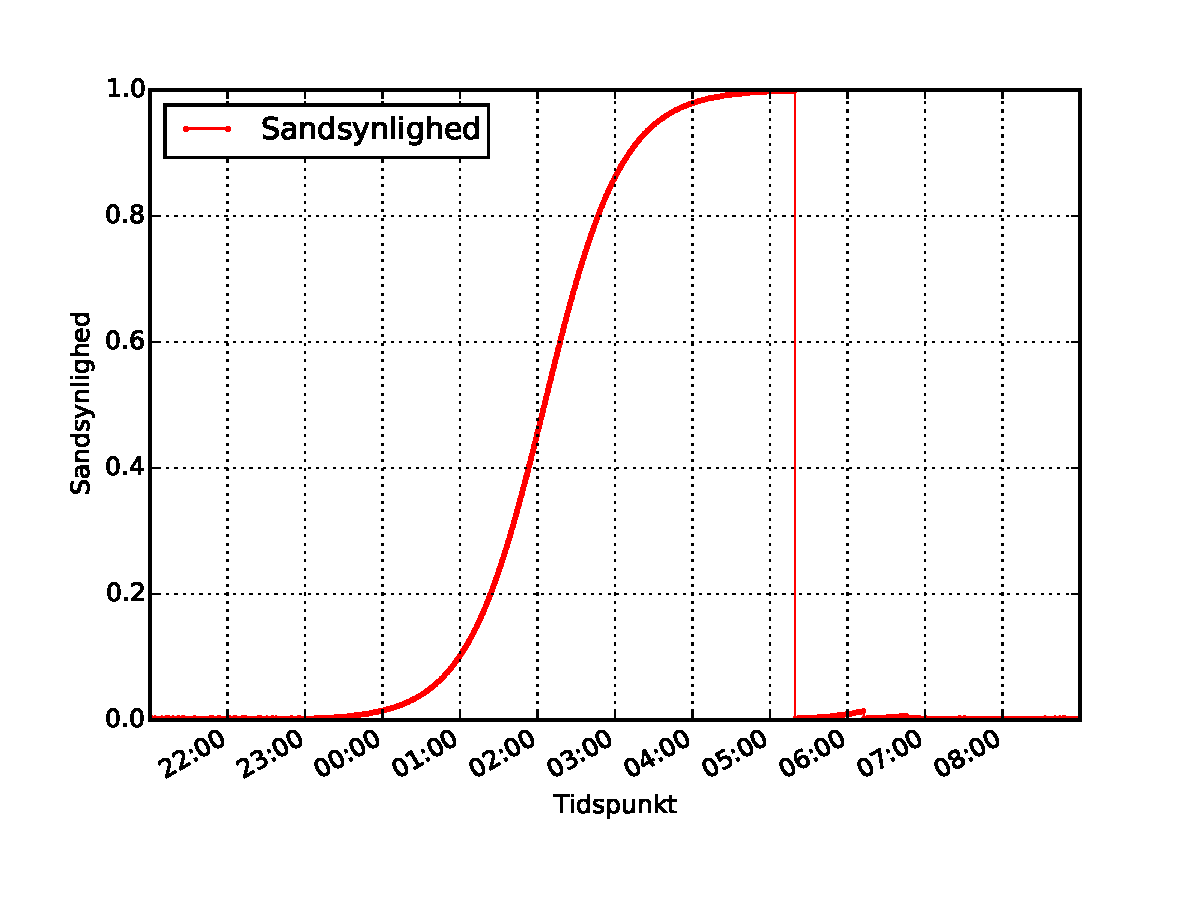
\includegraphics[scale=0.27, trim = 1cm 1cm 1cm 1cm, clip]{../Report/grafik/kombi_figur/amplitude-sleep-estimate-plot}
			\caption{Amplitude-søvnestimering.}
		\end{subfigure}
	\end{minipage}\\[1ex]%
\end{figure}

\end{frame}

\begin{frame}
\frametitle{Proof of concept}
Vi betragter stilstandsperioder som indikator på søvn.

\begin{figure}
	\begin{minipage}{\linewidth}
		\begin{subfigure}{0.32\linewidth}
			\centering
			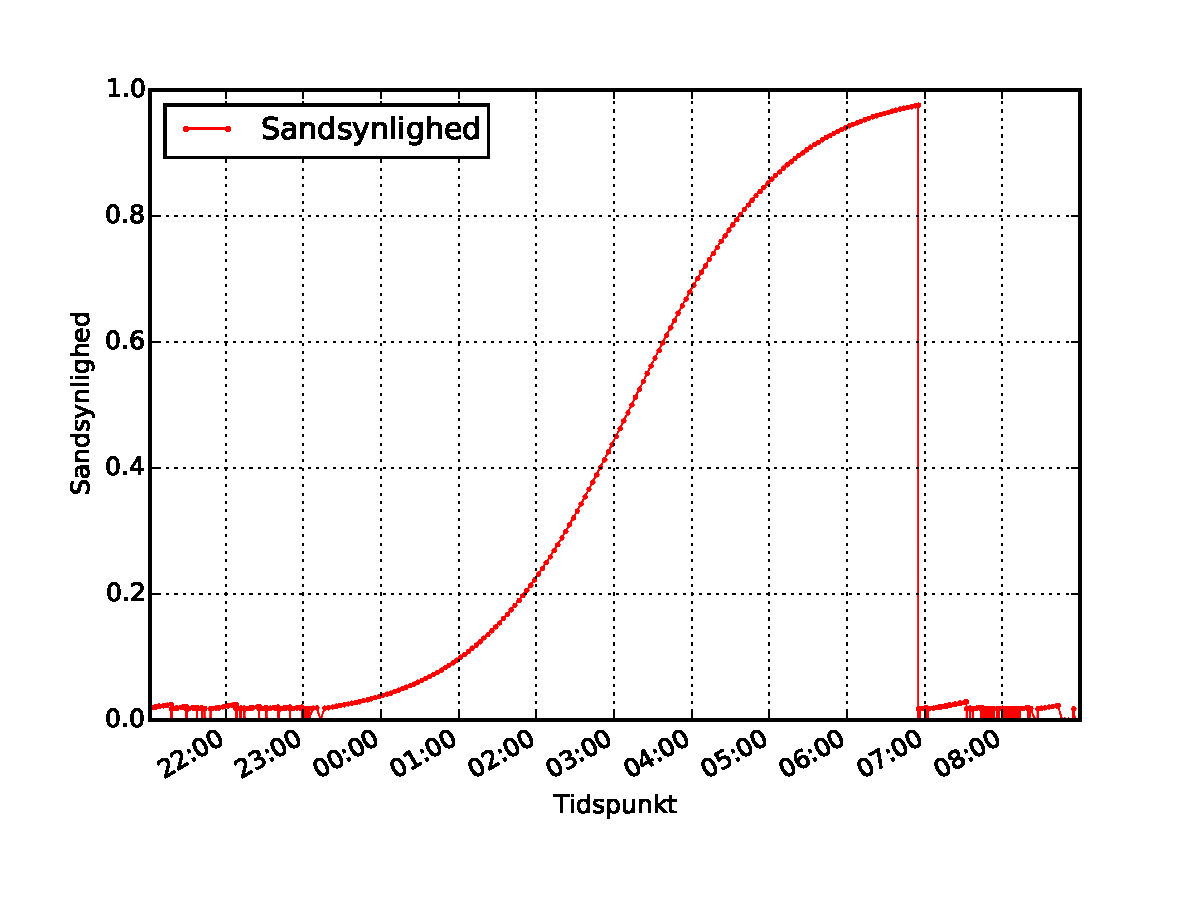
\includegraphics[scale=0.2, trim = 1cm 1cm 1cm 1cm, clip]{../Report/grafik/kombi_figur/acceleration-sleep-estimate-plot}
			\caption{Accelerations-søvnestimering.}\label{fig:sleepcalcaccplot}
		\end{subfigure}
		\begin{subfigure}{0.32\linewidth}
			\centering
			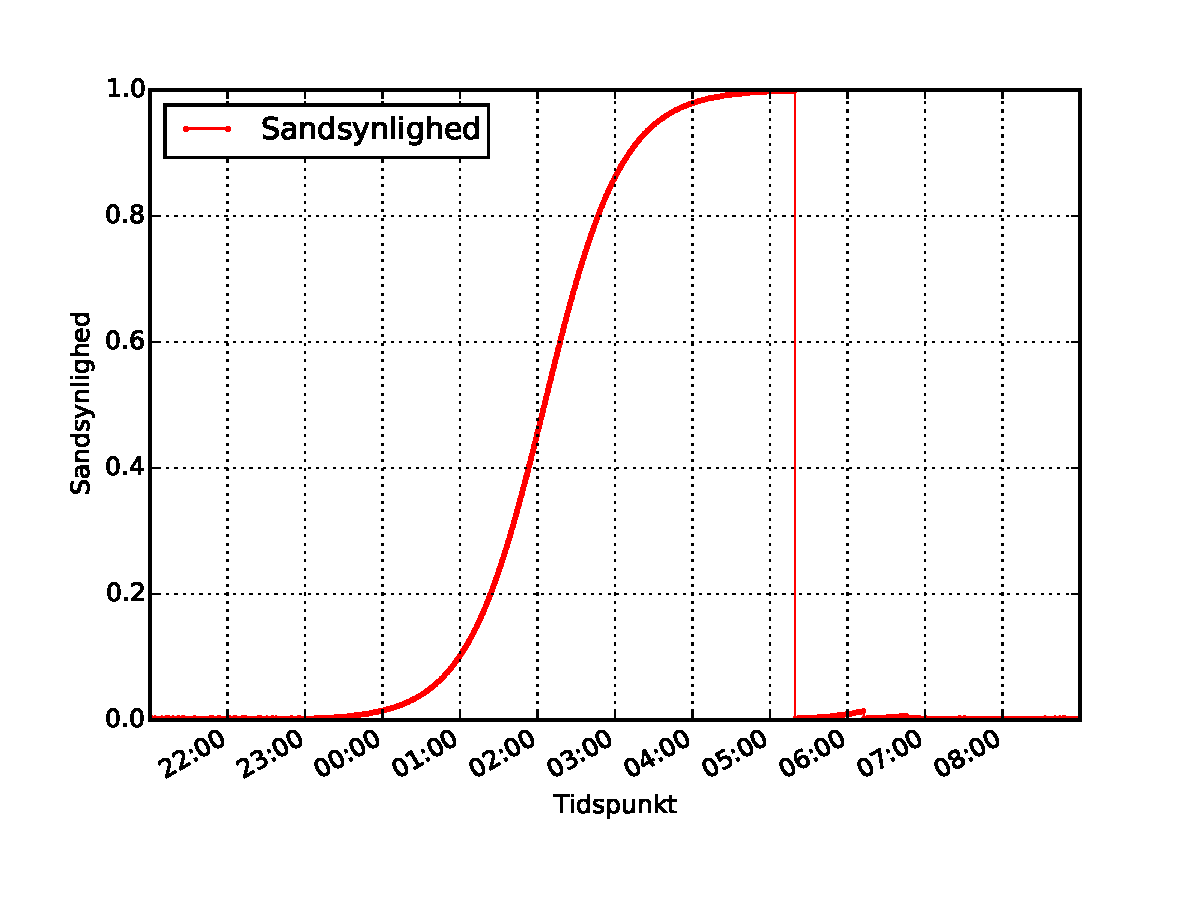
\includegraphics[scale=0.2, trim = 0cm 1cm 1cm 1cm, clip]{../Report/grafik/kombi_figur/amplitude-sleep-estimate-plot}
			\caption{Amplitude-søvnestimering}\label{fig:sleepcalcamplplot}
		\end{subfigure}
		\begin{subfigure}{0.32\linewidth}
			\centering
			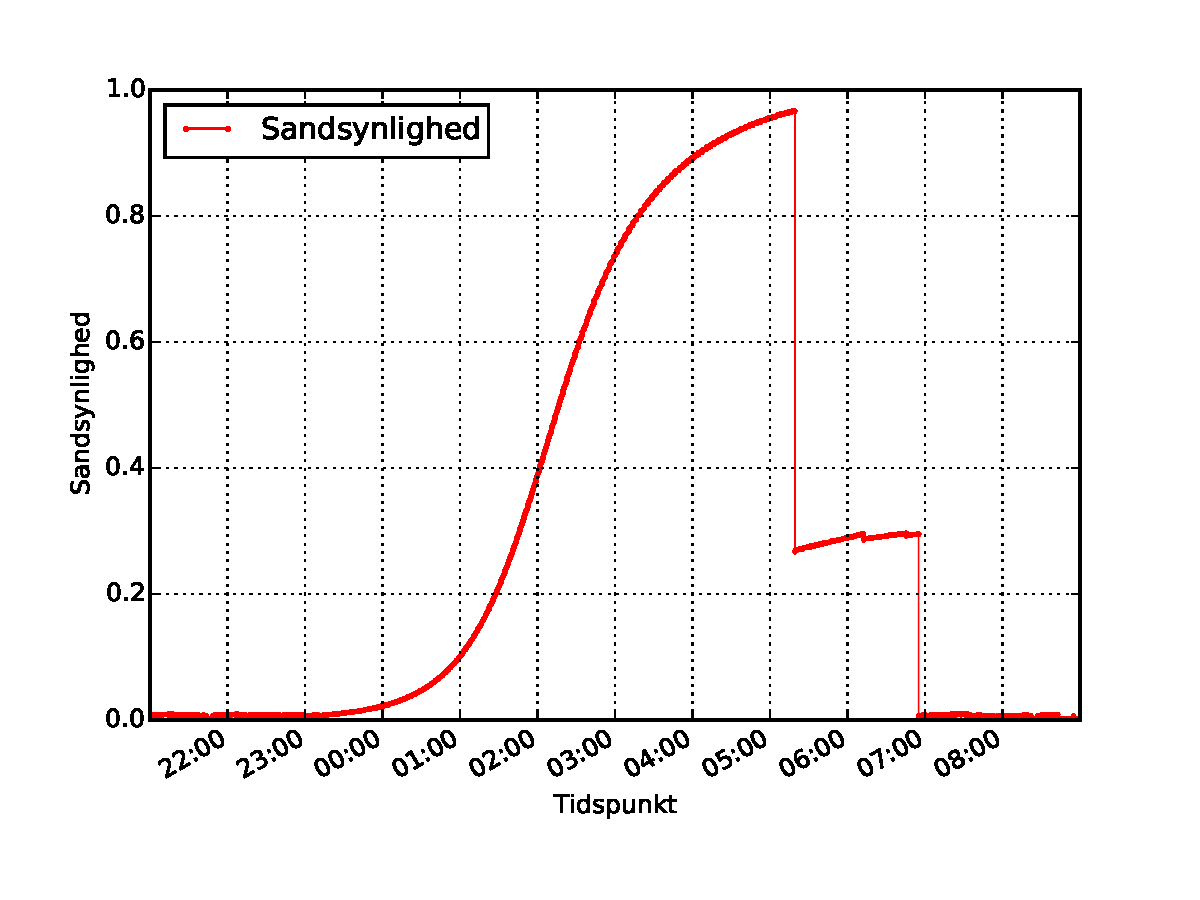
\includegraphics[scale=0.2, trim = 1cm 1cm 1cm 1cm, clip]{../Report/grafik/kombi_figur/combined-sleep-estimate-plot}
			\caption{Kombineret søvnestimering}\label{fig:sleepcalcombine}
		\end{subfigure}
	\end{minipage}\\[1ex]%
\end{figure}
\end{frame}

\begin{frame}
\frametitle{Proof of concept}
Vi betragter stilstandsperioder som indikator på søvn.

\begin{figure}
	\begin{minipage}{\linewidth}
		\begin{minipage}{\linewidth}
		
		\begin{subfigure}{\linewidth}
			\centering
			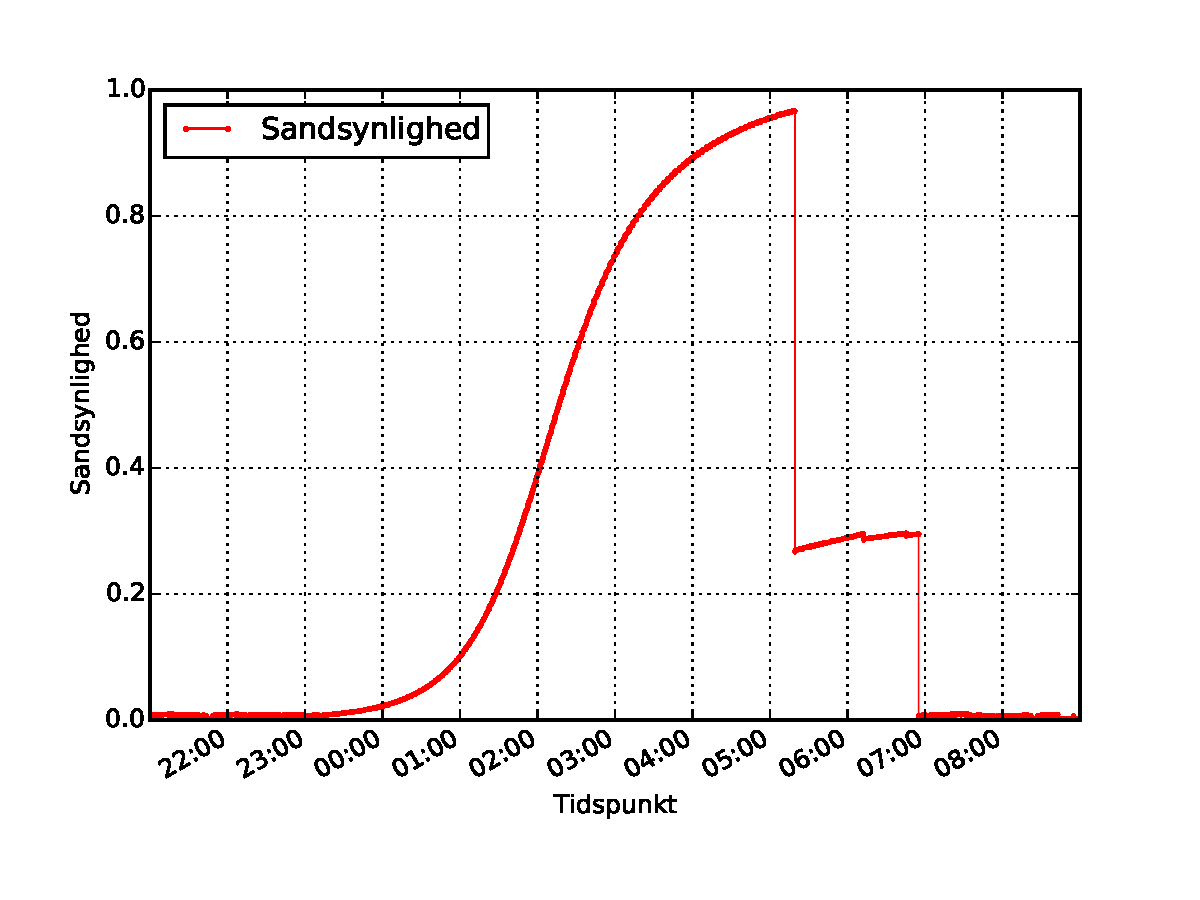
\includegraphics[scale=0.2, trim = 1cm 1cm 1cm 1cm, clip]{../Report/grafik/kombi_figur/combined-sleep-estimate-plot}
			\caption{Kombineret søvnestimering}\label{fig:sleepcalcombine}
		\end{subfigure}
		\end{minipage}
		\begin{minipage}{\linewidth}
		\begin{subfigure}{\linewidth}
			\centering
			\begin{tabular}{|c|c|c|}
			\hline starttid & sluttid & sandsynlighed \\ 
			\hline 2015-04-21 23:11 & 2015-04-22 05:19 & 0.97 \\ 
			\hline 2015-04-22 05:19 & 2015-04-22 06.45 & 0.29 \\ 
			\hline 
			\end{tabular}
			\caption{Samlet søvnaggregeringsresultat.}\label{fig:finalagg}
		\end{subfigure}
		\end{minipage}
	\end{minipage}\\[1ex]%
\end{figure}
\end{frame}

\section{Demonstration}
\begin{frame}
	%\frametitle{Demonstration}
	Demonstration
\end{frame}


\section{Refleksion og konklusion}
\begin{frame}
\frametitle{Refleksion og konklusion}
\begin{itemize}
	\item Kan vi benytte produktet udenfor psykiatrien?
	\item Vi har ikke begrænset os - mulighed for videreudvikling åben
	\begin{itemize}
		\item Bør arbejdes videre på
		\item Inddrage andre faktorer såsom snorken og fysisk aktivitet
		\item Nemt at udskifte metoden
	\end{itemize}
	\item Stammer vores data fra patienten eller en anden i husstanden?
	\begin{itemize}
		\item Centralt at vi måler præcist og på den rigtige hvis søvnestimering skal indgå i behandlingen
	\end{itemize}
	\item \textbf{Ændring i adfærd}
\end{itemize}
\end{frame}

\begin{frame}
\frametitle{Ændring i adfærd}

\begin{minipage}{0.54\linewidth}
	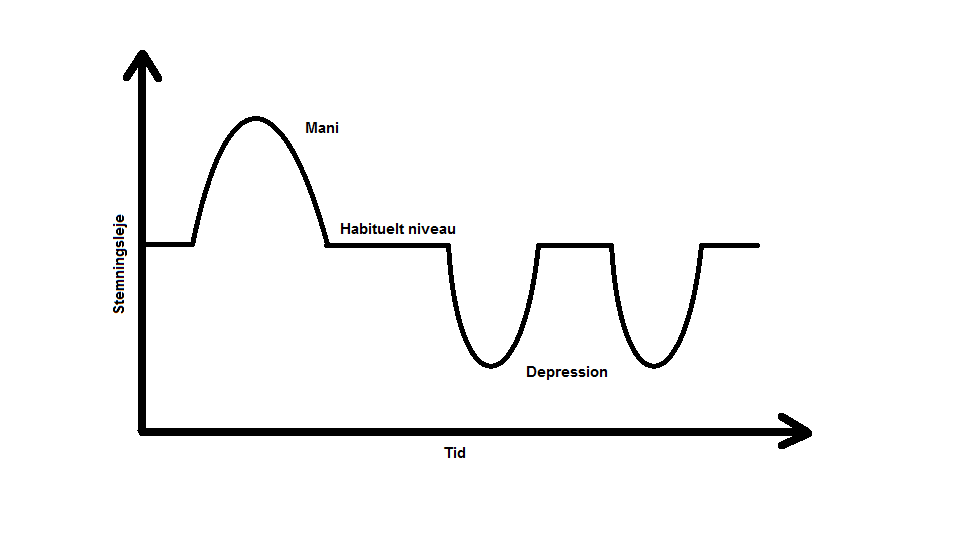
\includegraphics[scale=0.25]{affektivstemningsleje}
\end{minipage}
\begin{minipage}{0.45\linewidth}
	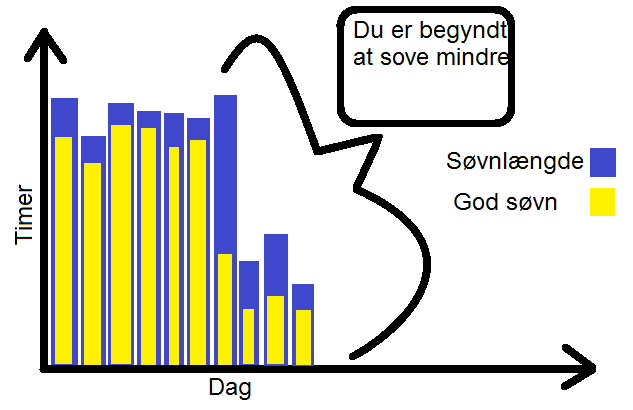
\includegraphics[scale=0.25]{soevnaendring}
\end{minipage}
\end{frame}

\bgroup
\setbeamercolor{background canvas}{bg=black}
\begin{frame}[plain]{}
\addtocounter{framenumber}{-1}	
	\begin{center}
	%\textcolor{white}{END}
	\end{center}
\end{frame}
\egroup
	
\end{document}
